\usepackage{greg}
\maketitle

\bgroup 

\section*{Abstract}\label{abstract}
\addcontentsline{toc}{section}{Abstract}

Homotopy type theory captures all the major concepts of differential
geometry including forms, connections, curvature, and gauge theory. We
show this by focusing on combinatorial manifolds, which are discrete in
the sense of real cohesion\cite{shulman_cohesion}, and drawing
inspiration from the similarly young field of discrete differential
geometry.

\egroup 

\begin{quote}
\centering

``It is always ourselves we work on, whether we realize it or not. There
is no other work to be done in the world.'' --- Stephen Talbott,
\emph{The Future Does Not Compute}\cite{talbott}
\end{quote}

\section{TODO}\label{todo}

After meeting with SA,MA 5/1/2024

\begin{itemize}
\item
  Focus on one audience: HoTT folks. Don't intermix as much classic
  geometry.
\item
  Section 1. Make explicit the triangle of DG, DDG, HoTT.
\item
  Section 2. Sphere example and combinatorial manifolds, torus example.
\item
  Section 3. Torsors and H-spaces
\item
  Poincaré-Hopf and/or Gauss-Bonnet, even just for some examples. The
  curvature will be given by loops around a circle via \(\Omega^2 f\)
  and the vector field will be integrated to an automorphism \(M\to M\)
  and some integer from there.

  \includegraphics{./968a77ed3382e1bbffa601a5a504c7759fb55e00.png}
\item
  Vector fields are sections of the disk bundle, which is the
  combinatorial neighborhood. We can define the circle bundle with our
  map to \(\BAutoso\) and add the base point to form the disk. Note that
  the requirement that every point have a link that is a simplicial
  sphere is called "combinatorial manifold" or "combinatorial
  triangulation".
\item
  When is a vector field an automorphism?
\item
  the disk bundle has a canonical section given by choosing the center
  point in each fiber. It has two other sections, one for each
  orientation of the circle.
\item
  At a fixed point of a vector field therefore, we can compare the
  vector field to either of the canonical sections. Use this to map to
  \(S^1\) or \(C_4\) or a path in one of those. This will have a winding
  number which is our index.
\item
  Prove that the total index is independent of a vector field that isn't
  the identity.
\item
  Prove Poincaré-Hopf
\end{itemize}

\section{Introduction: Discrete differential
geometry}\label{introduction-discrete-differential-geometry}

The observation that sparks the following discussion is this: if we can
manage to reformulate differential geometry in discrete terms (i.e.
finite, without infinitesimals) then we may also be able to construct it
synthetically in homotopy type theory. Furthermore, if we do capture
geometry in HoTT then there's a chance that it can become clearer and
smaller. We would then have new tools, a new audience, and a new program
to (re)explore geometry, gauge theory, low dimensional topology, and
mathematical physics.

Applied mathematicians and computer scientists have been developing
discrete differential geometry (DDG) for many years. The 2003 Ph.D.
thesis of Anil Hirani \cite{hiranidec} (see also the multi-author
follow-up \cite{desbrundec}) defines finite versions of vector fields,
differential forms, the wedge product, the Hodge star, and several
differential operators (exterior derivative, div, grad, curl,
Laplace-Beltrami, Lie derivative). Hirani and others cite Whitney's 1957
book \emph{Geometric Integration Theory}\cite{whitney1957} which
develops a theory of cochains by integrating smooth forms over chains.
In 2004 Melvil Leok, Jerrold Marsden, and Alan Weinstein \cite{leok}
defined discrete connections on principal bundles. This is probably the
work most spiritually similar to this paper. The motivation for the
above constructions was applied mathematics: modeling the differential
equations of mechanics and fluid mechanics with the so-called ``finite
element'' methods. The theory has been adopted and extended by the
computer graphics community as well (see Keenan Crane's course notes
\cite{crane_ddg} for a gentle survey).

The applied category theory community has begun to develop category
theoretic foundations and software libraries to increase the reusability
and compositionality of finite element methods in science and
engineering problems. See for example recent work to bring discrete
exterior calculus into the AlgebraicJulia library
\cite{morris_decapodes} \cite{patterson_diffeq}.

For these classically-minded applied mathematicians DDG is defined on
combinatorial manifolds such as simplicial complexes or polytopes, of
any finite dimension. The 0-cells play the role of points, the 1-cells
are path segments, and so on. They define \(n\)-forms as functions on
the \(n\)-dimensional faces of the manifold into the real numbers, which
is then extended by linearity to arbitrary \(n\)-chains. Exterior
differentiation is defined by Stokes theorem (which is no longer a
theorem in this setting), by which we mean the following.

\begin{mydef}
(Exterior derivative in DDG.) Let \( \omega \) be an \( n-1 \)-form on a combinatorial manifold \( M \), and let \( \Omega \) be an \( n \)-face of \( M \). Let \( \partial \) be the boundary operator on faces. The exterior derivative \( d \) is defined by 
\[ 
 d\omega(\Omega) = \omega(\partial\Omega).
\]
\end{mydef}

At this point a study of DDG would move into chain complexes, where the
forms of different dimensions are combined through the grading. Grassman
algebras would be introduced, to convey the dependence of forms on
orientation. The Leibniz rule (product rule) would be explored. Defining
connections and curvature require constructing a codomain that is
group-like and then creating more definitions about transport and
holonomy. At that point major theorems like Gauss-Bonnet and Chern-Weil
would be available to prove.

We will take a different path. We will not define forms, complexes, or
Grassman algebras at all. We will view ordinary HoTT functions out of a
type as \emph{synthetic discrete differential forms}. The codomain will
be a central H-space, which combines the features of the real numbers
(in that functions can be pointwise multiplied) and classifying spaces
of groups (so that maps into the H-space can classify bundles). We will
then merely \emph{observe} the emergence of various aspects of geometry.

We won't be able to answer every question, so eventually we will stop
and point to future directions.

\section{Examples}\label{examples}

\subsection{The tangent bundle of the
2-sphere}\label{the-tangent-bundle-of-the-2-sphere}

\begin{itemize}
\item
  Define \(\oo\) via skeleta with inclusions. Use the inclusions to help
  identify aspects of the map \(\oo\to\BAutoso\).
\item
  Make it a lemma that \(\oo\) is the triple join
\item
  Define polytopes
\end{itemize}

The usual HoTT \(S^1\) and \(S^2\) are a little impoverished, and seeing
connections and curvature is difficult. Instead we will define
equivalent HITs that have more constructors. The representation of the
sphere will be the octohedron \(\oo\) and the circle will be \(C_4\)
which has four points and is designed to work well with \(\oo\).

The Rubik's cube has a convenient standardized arrangement of colors
that start with different letters (white, yellow, blue, orange, green,
red) so we will use those to label our points, especially since having
such a cube handy is very helpful to visualize some of the geometry that
is encoded below as mere lists of data.

Should the 0-dimensional constructors represent the corners or the
faces? We have so far found it intuitive to imagine taking the nerve of
a good open cover, where the top-dimensional bulk of the cube, namely
the faces, is converted to a point since an open set covering that face
is contractible. That's why we end up with an icosohedron, which is a
dual polyhedron to the cube.

We won't discuss in detail the fact that Mike Shulman's shape operator
\cite{shulman_cohesion} is equivalent to taking the nerve of an open
cover and forming a HIT from the overlap data. The shape operator
preserves colimits and so the simple homotopy pushouts we are
considering should be within the use cases of shape.

The HIT \(\oo\) is built from the following constructors:

\begin{enumerate}
\item
  Dimension 0: the vertices \(\{w, y, b, g, r, o, y\}\) where we think
  of \(w\) as the north pole and \(y\) the south pole.
\item
  Dimension 1: the 12 adjacency pairs of faces, denoted
  \(\{wb\}, \{wo\}\) and so on.
\item
  Dimension 2: the set of faces generated by the 3-way adjacency of
  faces (which takes place in neighborhoods of the cube's original
  corners), denoted \(\{wbo\}, \{wog\}\) and so on.
\end{enumerate}

\begin{figure}
\centering
\begin{minipage}[t]{0.45\linewidth}
\centering
\end{minipage}
\hfill
\begin{minipage}[t]{0.45\linewidth}
\includegraphics{./ff7f3a1e9ad288427a1f8fe354f5e5e4112b62fd.png}
\end{minipage}
\caption{The HIT \(\oo\) which has 6 points, 12 1-paths, 8 2-paths.}
\end{figure}

We will choose a base point of \(\BAutoso\) that has four points, just
like the equator of \(\oo\).

\begin{mydef}
Denote by \( C_4 \) the join \( \{b, g\}*\{r, o\} \). This is the equator of the discrete octahedral sphere. Then \( \oo \) itself can be seen as the join \( \{w, y\}* C_4 \).
\end{mydef}

\begin{figure}
\centering
\begin{minipage}[t]{0.45\linewidth}
\centering
\end{minipage}
\hfill
\begin{minipage}[t]{0.45\linewidth}
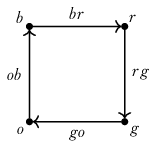
\includegraphics{./45744937ac561c6ce05f971621a980d63ad6d2e1.png}
\end{minipage}
\caption{The HIT \(C_4\) which is one of the types in \(\BAutoso\)}
\end{figure}

\begin{mylemma}
\( (C_4, b)\simeq S^1 \).
\end{mylemma}

\emph{Proof.} Similar to Lemma 6.5.1 from the HoTT book\cite{hottbook}.
We will make some use of the particular map
\(\{b, r, g, o\}\mapsto \mathsf{base}, br\mapsto \mathsf{loop}, \{rg, go, ob\}\mapsto \refl.\)~◻

\begin{mylemma}
\( \oo\simeq S^2 \).
\end{mylemma}

\emph{Proof.} \(\oo\) is the join of \(C_4\) and a two-point type. For
more discussion of the join operation see the HoTT book section
8.5\cite{hottbook}.~◻

To produce a term in \(\BAutoso\) we need \(C_4\) and a choice of an
equivalence class of equivalences with \(S^1\):

\begin{mylemma}
We have \( (C_4, ||\{b, r, g, o\}\mapsto \mathsf{base}, br\mapsto \mathsf{loop}, \{rg, go, ob\}\mapsto \refl ||_0):\BAutoso \)
\end{mylemma}

There are other near-to-hand terms of \(\BAutoso\) we can denote like:
\([w, o, y, r]\), meaning the square isomorphic to \(C_4\) but with the
given four points, with pointing given by whichever point we listed
first, and with equivalence with \(S^1\) chosen so that the path between
the first two points maps to \(\mathsf{loop}\). We will also introduce
notation for maps \(f:[a, b, c, d]\to [w, x, y, z]\) by indicating where
each item in the domain list is sent, like so:
\(f\defeq[[x, y, z, w]]\).

\(C_4\) has an unpointed automorphism connected to the identiy which
will play the role of rotation by 90 degrees:

\begin{mydef}
Let \( R:C_4\to C_4 \) be the cyclic permutation given by \( R(b)=r, R(r)=g, R(g)=o, R(o)=b, R(br)=rg, R(rg)=go, R(go)=ob, R(ob)=br. \) Let \( R':R=\id \) be the obvious homotopy to the identity.
\end{mydef}

To construct a map \(\oo\to\BAutoso\) we need to send each vertex to an
\(S^1\)-torsor such as \(C_4\). We will choose to send each vertex to
``the clockwise equator if this was the north pole.''

\begin{figure}
\centering
\begin{minipage}[t]{0.225\linewidth}
\centering
\end{minipage}
\hfill
\begin{minipage}[t]{0.225\linewidth}
\includegraphics{./5223124258db050f495250e281a65d462714f6df.png}
\end{minipage}
\hfill
\begin{minipage}[t]{0.225\linewidth}
\includegraphics{./f8ad0fbb66a7ad51b3cb4db7a0f35ea8a8a56a4b.png}
\end{minipage}
\hfill
\begin{minipage}[t]{0.225\linewidth}
\includegraphics{./d3b55304a407c9ca808e19bf9256206529608d82.png}
\end{minipage}
\caption{The equators for \(w, b, r\).}
\end{figure}

\begin{mydef}
Define \( T_0:\oo\to\BAutoso \) on just the 0-skeleton by
\begin{itemize}
\item \( T_0(b)=[w, o, y, r] \).
\item \( T_0(o)=[w, g, y, b] \).
\item \( T_0(g)=[w, r, y, o] \).
\item \( T_0(r)=[w, b, y, g] \).
\item \( T_0(w)=[b, r, g, o] \).
\item \( T_0(y)=[b, o, g, r] \).
\end{itemize}
\end{mydef}

Extending this to the 1-skeleton requires various choices. We will
choose the one that reflects the tangent bundle, using the transport we
can intuitively see through the embedding of \(\oo\) in 3-dimensional
space as in our pictures. If you focus for a moment just on a path
\(w\to b\to r\) and imagine rigidly tipping a moving equator along with
a moving point, you can imagine a moving-equator point that starts at
\(r\) and stays fixed when the north pole slides from \(w\) to \(b\).
When the north pole continues sliding from \(b\) to \(r\) the
moving-equator point moves to \(g\). Then it remains fixed when the
north pole slides from \(r\) up to \(w\). So all in all we ``moved \(r\)
to \(g\).'' When we track all the points on the original \(w\)-equator
we see that we performed the rotation we earlier named \(R\).

In general we have:

\begin{mydef}
Define \( T_1:\oo\to\BAutoso \) on just the 1-skeleton by extending \( T_0 \) as follows:
Transport away from \( w \):
\begin{itemize}
\item \( T_1(wb):[b, r, g, o]\mapsto [y, r, w, o] \) (\( r, o \) fixed)
\item \( T_1(wr):[b, r, g, o]\mapsto [b, y, g, w] \) (\( b, g \) fixed)
\item \( T_1(wg):[b, r, g, o]\mapsto [w, r, y, o] \)
\item \( T_1(wo):[b, r, g, o]\mapsto [b, w, g, y] \)
\end{itemize}
Transport away from \( y \):
\begin{itemize}
\item \( T_1(yb):[b, o, g, r]\mapsto [w, o, y, r] \)
\item \( T_1(yr):[b, o, g, r]\mapsto [b, y, g, w] \)
\item \( T_1(yg):[b, o, g, r]\mapsto [y, o, w, r] \)
\item \( T_1(yo):[b, o, g, r]\mapsto [b, w, g, y] \)
\end{itemize}
Transport along the equator:
\begin{itemize}
\item \( T_1(br):[w, o, y, r]\mapsto [w, b, y, g] \) 
\item \( T_1(rg):[w, b, y, g]\mapsto [w, r, y, o] \)
\item \( T_1(go):[w, r, y, o]\mapsto [w, g, y, b] \)
\item \( T_1(ob):[w, g, y, b]\mapsto [w, o, y, r] \)
\end{itemize}
\end{mydef}

At this point we have defined a map on the 1-skeleton of \(\oo\).

\begin{myclaim}
\( T_1 \) defines a principal circle bundle with connection over the 1-skeleton of \( \oo \).
\end{myclaim}

We now want to extend this map to all of \(\oo\) by providing values for
the eight faces. Here we will be guided by the classical relationship
between a connection and its curvature. The curvature is computed from
the connection, it doesn't contain any new data. Classically the
integral of curvature over a 2-cell is the holonomy given by transport
around the boundary.

\begin{mydef}
Define \( T_2:\oo\to\BAutoso \) by extending \( T_1 \) as follows. We will send every clockwise triangle to \( R' \), the homotopy from \( \refl \) to \( R \):
\begin{itemize}
\item \( T_2(wbr)=R' \) 
\item \( T_2(wrg)=R' \)
\item \( T_2(wgo)=R' \)
\item \( T_2(ybo)=R' \)
\item \( T_2(yrb)=R' \) 
\item \( T_2(ygr)=R' \)
\item \( T_2(yog)=R' \)
\item \( T_2(ybo)=R' \)
\end{itemize}
\end{mydef}

\subsection{Combinatorial manifolds}\label{combinatorial-manifolds}

(This section is not quite off the ground.)

The combinatorial structure we have in mind is a nerve of a good open
cover. What do we know about which smooth manifolds have such covers?
While we're at it, let's survey all the combinatorial-flavored spaces
and survey what smooth manifolds are homotopy equivalent to which
structures.

What topological manifolds are equivalent to a CW complex? The answer is
the composition of a few results summarized by Allen Hatcher\footnote{\url{https://mathoverflow.net/questions/201944/topological-n-manifolds-have-the-homotopy-type-of-n-dimensional-cw-complexes}}
(citing \cite{kirby_siebenmann} and \cite{freedman_quinn}):

\begin{quote}
Every topological manifold has a handlebody structure except in
dimension 4, where a 4-manifold has a handlebody structure if and only
if it is smoothable. This is a theorem on page 136 of Freedman and
Quinn's book ``Topology of 4-Manifolds'', with a reference given to the
Kirby-Siebenmann book for the higher-dimensional case. It is then an
elementary fact that an \(n\)-manifold with a handlebody structure is
homotopy equivalent to a CW complex with one \(k\)-cell for each
\(k\)-handle, so in particular there are no cells of dimension greater
than \(n\). At least in the compact case a manifold with a handlebody
structure is in fact homeomorphic to a CW complex with \(k\)-cells
corresponding to \(k\)-handles; see page 107 of Kirby-Siebenmann. This
probably holds in the noncompact case as well, though I don't know a
reference.
\end{quote}

\section{Central H-spaces}\label{central-h-spaces}

\begin{itemize}
\item
  introduce torsors
\item
  show subtlety how \(BG\) doesn't classify stuff since it has extra
  properties
\item
  draw

  \includegraphics{./6a4feec92d142f0ad0daeaca4306a46f9aaa33a5.png}
\item
  H-spaces paper result equating this to a universal cover of a
  component of the universe. (It should feel significant that
  \(BS^1\simeq \BAutoso\).)
\end{itemize}

Central H-spaces are the classifying spaces for principal bundles on
abelian groups. We won't be able to access the full theory for
nonabelian groups just yet, but we hope that the theory of maximal tori
and weights might bring even those within reach of the central H-space
paradigm.

We will rely on the lovely paper by Buchholtz, Christensen, Flaten and
Rijke \cite{buchholtz2023central}.

\begin{mydef}
An H-space structure on a pointed type \( (B,b) \) consists of
\begin{enumerate}
\item A binary operation \( \mu:B\to B\to B \)
\item A left unit law \( \mu_l:\mu(\pt,-)=\id_B \)
\item A right unit law \( \mu_r:\mu(-,\pt)=\id_B \)
\item A coherence \( \mu_{lr}:\mu_l(\pt)=_{\mu(\pt,\pt)=\pt}\mu_r(\pt) \)
\item A proof of left- and right- invertibility: \( \mu(a,-):A\simeq A \), \( \mu(-, b):A\simeq A \)
\end{enumerate}
\end{mydef}

\begin{myprop}
(\cite{buchholtz2023central} Prop 3.6) Let \( A \) be a pointed type. Then the following are equivalent:
\begin{enumerate}
\item \( A \) is central.
\item \( A \) is a connected H-space and \( A\dotto A \) is a set.
\item \( A \) is a connected H-space and \( A\simeq A \) is a set.
\end{enumerate}
\end{myprop}

This result will inform our study of the Leibniz rule: the analogue of
the algebra of functions to \(\rr\) is:

\begin{myprop}
For any type \( M \) and H-space \( B \) the type of maps \( M\to B \) with base point the constant map is an H-space under pointwise multiplication.
\end{myprop}

We will also be looking in detail at maps into the classifying space of
\(S^1\) bundles. The Buchholtz et al paper\cite{buchholtz2023central}
describes this type in several helpful ways, summarized by:

\begin{mythm}
For any central H-space \( A \) (such as \( S^1 \)) the type of torsors of \( A \) is a delooping of \( A \), and is equivalent to \( \BAut_1(A)\defeq \sit{X:\U}||X=A||_0. \) This delooping is also a central H-space and so can be infinitely delooped.
\end{mythm}

This means that we can form a sequence of deloopings
\(\zz, S^1, \BAutoso, \ldots\).

\section{Why this is geometry}\label{why-this-is-geometry}

How can we double check that we are describing the intended theory of
geometry? In this section we will enumerate a wishlist of facts that we
believe characterize the subject, and then provide evidence for some of
them.

Here are the translations that are covered in the current paper:
\[\begin{aligned}
& \text{\small Connections are infinitesimal splittings of a} & \quad &\text{\small Paths in a sigma type are equivalent to a}        \\
& \text{\small principal bundle.} & \quad&\text{\small pair of paths.}        \\ \hline
& \text{\small Differentials satisfy the Leibniz (product) rule.} &\quad  &\text{\small Horizontal composition in an H-space is} \\ 
&  &  \quad&\text{\small performed in two steps.} \\ \hline
& \text{\small Connections with 0-truncated groups are covering}        &\quad &\text{\small Transport around contractible loops is } \refl             \\ 
& \text{\small spaces with unique flat connection.}        & \quad&\text{\small when fibers are sets.}             \\ \hline
& \text{\small The group of gauge transformations (bundle} &\quad &\text{\small Homotopies of classifying maps respect } \\ 
& \text{\small automorphisms) acts on the space of connections.} & \quad&\text{\small the splitting of paths in sigma types.} \\ 
\end{aligned}\]

And here are questions to explore in the future:

\begin{enumerate}
\item
  There's a notion of \emph{tensorial} that holds for forms but not for
  connections.
\item
  Where is the Grassmannian structure of wedge product?
\item
  The Gauss-Bonnet theorem holds, relating the curvature of a 2-manifold
  to the Euler characteristic.
\item
  More generally, characteristic classes of bundles can be computed
  using a connection (Chern-Weil theory).
\end{enumerate}

\subsection{Higher maps contain
connections}\label{higher-maps-contain-connections}

To hew close to the intended context of the term ``connection'' we will
examine manifold-like types mapping into bundle-classifying-like types.
The novelty here, compared to other HoTT investigations, is the focus on
combinatorial types to stand in for manifolds.

In recent times it has been believed in the HoTT community that maps
from a discrete type to a discrete classifying space can encode only the
connections that a classical mathematician would call \emph{flat} (zero
curvature). In this context the word \emph{discrete} means having the
discrete topology, in the sense of cohesion\cite{shulman_cohesion}. This
is not the case! We will show that if the codomain is a classifying
space of \(S^1\) or other group of homotopy dimension at least 1, then
non-flat connections appear despite the type \(S^1\) being topologically
discrete. Another common meaning of the shorthand ``discrete'' is to
indicate a 0-truncated type, i.e. a set, as opposed to a type with
higher homotopical structures. We will show that indeed if the codomain
classifies sets, which is the case for example with the classifying
space \(B\zz\), the delooping of \(\zz\), then connections are flat.
(The type we denote by \(\mathbb{S}^1\defeq\{(x, y)|x^2+y^2=1\}\) is a
set and is not topologically discrete. We will not be discussing it at
all in this paper.)

The DDG philosophy tells us to look at HITs that are polytope-like. A
polytope \(M\) will have finitely many 0-dimesional (point) constructors
\(\{m_0^i\}\), finitely many 1-dimesnional constructors
\(\{m_1^{ij}:m_0^i=m_0^j\}\), and so on. Type families \(f:M\to \U\) on
this type specify where each of these constructors is sent. In DDG
parlance, \(f\) restricted to the 0-dimensional constructors of \(M\) is
a 0-form and \(f\) restricted to the 1-dimensional constructors (not the
1-skeleton but just the 1-dimensional parts, whatever that means in
HoTT) is a 1-form, and so on.

A principal \(S^1\) bundle is a family of \(S^1\) torsors and so we will
often be focusing on the function type \(M\to \BAutoso\). The novel
claim here is that \(M\to \BAutoso\) contains more than just all the
principal \(S^1\)-bundles: it also contains all the connections on all
the bundles. Every connection is present, both curved and flat, because
we have complete freedom to specify the images of the paths.

Classically, curvature is a property of the connection. It is computed
either on infinitesimal loops, or on the infinitesimal surface bounded
by the loop. In fact it is ``the derivative of the connection'' morally
speaking. Getting into the details would wreck the simplicity we're
going for\footnote{I'm picking and choosing where to tell the story
  fully twice (see the next section) and where to simply look for
  motivation.}. We will look for curvature by examining \(f\) on
1-dimensional loops. If \(M\) is at least a 2-type and if we want to
claim that \(f\) classifies a bundle with connection, then we will be
required to map the 2-faces of \(M\) (the 2-dimesional constructors) to
a path from \(\refl\) to the image of a bounding loop. So at dimension 2
we will impose that constraint. Since \(\BAutoso\) is 2-truncated, \(f\)
factors through the truncation map \(M\to||M||_2\) and so that's the top
dimension.

There is an example at the end of this paper. For those who are best
served by examples, do look at it and return to this point.

\subsection{Connections as splittings}\label{connections-as-splittings}

The classical story goes like this.

\begin{mydef}
The \emph{vertical bundle} \( VP \) of a principal bundle \( \pi:P\to M \) with Lie group \( G \) is the kernel of the derivative \( T\pi:TP\to TM \). 
\end{mydef}

\(VP\) can be visualized as the collection of tangent vectors that point
along the fibers. It should be clear that the group \(\Aut P\) acts on
\(VP\): an automorphism \(\phi:P\to P\) sends \(V_pP\) to
\(V_{\phi(p)}P\), where of course \(\pi(p)=\pi(\phi(p))\).

\begin{mydef}
An \emph{Ehresmann connection} on a principal bundle \( \pi:P\to M \) with Lie group \( G \) is a splitting \( TP=VP\oplus HP \) at every point of \( P \) into vertical and ``horizontal'' subspaces, which is preserved by the action of \( \Aut P \).
\end{mydef}

Being preserved by the action of \(\Aut P\) means that the complementary
horizontal subspaces in a given fiber of \(\pi:P\to M\) are determined
by the splitting at any single point in the fiber. The action of \(G\)
on this fiber can then push the splitting around to all the other
points.

The motivation for this definition is that we now have an isomorphism
\(T_p\pi:H_pP\to T_{\pi(p)}M\) between each horizontal space and the
tangent space below it in \(M\). This means that given a tangent vector
at \(x:M\) and a point \(p\) in \(\pi^{-1}(x)\) we can uniquely lift the
tangent vector to a horizontal vector at \(p\). We can also lift vector
fields and paths in this way. To lift a path \(\gamma:[0,1]\to M\) you
must specify a lift for \(\gamma(0)\) and then lift the tangent vectors
of \(\gamma\) and prove that you can integrate the lift of that vector
field upstairs in \(HP\).

Then, armed with the lifting of paths one immediately obtains
isomorphisms between the fibers of \(P\). So the Ehresmann connection,
the lifting of paths, and transport isomorphisms between fibers are all
recapitulations of the structure that the connection adds to the bundle.

Moving now to HoTT, fix a type \(M:\U\) and a type family \(f:M\to\U\).
Path induction gives us the transport isomorphism
\(\pit{p:x=_M y}\tr(p):f(x)=f(y)\). We can use this to define a type of
\emph{dependent paths}, also called \emph{pathovers} or \emph{paths
over} a given path.

\begin{mydef}
With the above context and points \( a:f(x), b:f(y) \) the type of \emph{dependent paths over \( p \)} with endpoints \( a, b \) is denoted
\[ a\pathover{p}b.
\]
By induction we can assume \( p \) is \( \refl_a \) in which case \( a\pathover{p}b \) is \( a=_{f(x)}a \).
\end{mydef}

See \cite{Symmetry} for more discussion of dependent paths (where they
use the term ``path over''), including composition, and associativity
thereof.

We recall now the identity type of sigma types:

\begin{mythm}\label{thm:idsit}
(HoTT book Theorem 2.7.2 \cite{hottbook}) If \( f:M\to \U \) is a type family and \( w,w':\sit{x:M}f(x) \) then there is an equivalence 
\[ 
\mathsf{split}:(w=w')\simeq \sit{p:\pr_1(w)=_M\pr_1(w')} \left[\tr(p)(\pr_2(w))\right] = \pr_2(w').
\]
\end{mythm}

In particular, given \(p:x=_M y\) and \(w:f(x)\) we have
\(w\pathover{p}tr(p)(w)\simeq tr(p)(w)=_{f(y)}tr(p)(w)\) which has the
term \(\refl\) which we can call ``the horizontal lift of \(p\) starting
at \(w\).'' We can imitate the classical definition of a connection by
defining \(\omega\defeq \pr_2\circ\mathsf{split}\), the projection onto
the vertical component. And thus in HoTT we can see the equivalence of
transport and lifting of paths into horizontal and vertical components.

\subsection{The Leibniz (product) rule}\label{the-leibniz-product-rule}

The Leibniz rule for exterior differentiation states that if
\(f, g:M\to \rr\) are two smooth functions to the real numbers then
\(d(fg) = fdg + gdf\). Here \(fg\) is the function formed by taking the
pointwise product of \(f\) and \(g\). This is an interaction between
multiplication in \(\rr\) and the action on vectors of smooth functions
(the 1-forms \(df\) and \(dg\)).

To examine this situation in HoTT we need type-theoretic functions
\(f, g:M\to B\) from some type \(M\) to a central H-space \(B\). Let
\(\mu:B\to B\to B\) be the H-space multiplication. How does \(\mu\) act
on paths? Suppose we have \(a, a', b, b':B\) and
\(p:a=_B a', q:b=_B b'\). Then we also have homotopies
\(\mu(p, -):\mu(a, -)=_{B\to B}\mu(a', -)\) and
\(\mu(-,q):\mu(-,b)=_{B\to B}\mu(-,b').\) Since \(\mu(a, -):B=B\) is an
(unpointed) equivalence of \(B\), and similarly for \(\mu(b, -)\) and so
on, this data assembles into the following diagram of higher groupoid
morphisms:

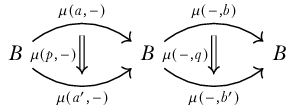
\includegraphics{./d183777157a8a3e2d296890f77fb0c2aee7abf41.png}

And so the two homotopies can be horizontally composed to give a path
\[\mu(p,-)\star\mu(-,q): \mu(a, b)=\mu(a',b').\] Horizontal composition
is given by
\[\mu(p,-)\star\mu(-,q)\defeq(\mu(p,-)\cdot_r \mu(-,b))\cdot(\mu(a', -)\cdot_l\mu(-, q))\]
where \[\mu(p,-)\cdot_r\mu(-,b):\mu(a,b)=\mu(a',b)\] and
\[\mu(a',-)\cdot_l\mu(-,q):\mu(a',b)=\mu(a',b')\] are defined by path
induction. See the HoTT book Theorem 2.1.6 on the Eckmann-Hilton
argument\cite{hottbook}.

We can recognize the process of using whiskering to form horizontal
composition in the Leibniz rule.

Quick aside: moving from infinitesimal calculus to finite groupoid
algebra actually involves two changes. The first is the change from
vectors to paths, forms to functions and so on. But it's also the case
that tangent vectors have just the one basepoint, whereas paths have two
endpoints. You can see this play out in this example, where \(a\) and
\(a'\) were distinct points (and \(b\) and \(b'\)).

The horizontal composition we build lives entirely in \(B\) and we
didn't make use of \(M\) yet. The Leibniz rule will be a pointwise
version of what's going on in \(B\). Denote by \(\mu\circ(f,g):M\to B\)
the map which sends \(x\mapsto \mu(f(x),g(x))\).

\begin{mylemma}
Given \( f, g:M\to B \) and \( p:x=_M y \) then 
\begin{align*}
 \ap(\mu\circ(f,g))(p)&=\mu(f(p),-)\star\mu(-,g(p))\\
 &=\left[\mu(f(p),-)\cdot_r \mu(-,g(x))\right]\cdot \left[\mu(f(y),-)\cdot_l\mu(-,g(p))\right]\\
 &:\mu(f(x),g(x))=\mu(f(y),g(y))
\end{align*}
\end{mylemma}

\subsection{Covering spaces}\label{covering-spaces}

If \(G\) is a 0-truncated group such as \(\zz\) then the type of torsors
(delooping) \(BG\) is 1-truncated. If \(f:M\to BG\) is a type family
then \(\sit{x:M}f(x)\) has fibers that are sets (\(G\)-torsors). So
transport functions are set isomorphisms, and the transport of any
contractible loop in \(M\) will be \(\refl\) (the identity) of the
fiber, which is what we mean by flat.

\subsection{Gauge transformations}\label{gauge-transformations}

A \emph{gauge transformation} is a term inherited from physics. It's an
automorphism of a principal bundle \(P\to M\), meaning a homeomorphism
of \(P\) that commutes with the projection to \(M\) and so acts on each
fiber. It is further required to be equivariant under the action of the
group \(G\), and so it's very similar to the act of multiplying each
fiber by a continuously varying element of \(G\).

In HoTT if the bundle is classified by \(f:M\to \U\) then an
automorphism is a homotopy \(f\sim f\) and the group of gauge
transformations is the loop space \(\Omega_f(M\to \U)\).

Recall that torsors have a physical interpretation as a quantity without
a specified unit, such as mass, length, or time. When we choose a base
point in a torsor it becomes the standard torsor \(G\) acting on itself
(for example, the additive real numbers). A physicist is looking for
properties or laws that are independent of such a choice. In the 20th
century physicists further wondered about choices of units that vary
from point to point, and began searching for laws that are invariant
under this much larger space of transformations. And so they and we are
led to explore quotienting by the action of the group of gauge
transformations, and in particular the space of connections ``mod
gauge.'' In this scenario the base manifold \(M\) is spacetime, and a
gauge transformation is a smoothly varying choice of gauge (units) at
each point.

Gauge transformations act on connections. When we view connections as
infinitesimal splittings of \(TP\) into vertical and horizontal
sub-bundles, a gauge transformation that is constant in the neighborhood
of a point will not change the splitting, it will just shift the fiber
rigidly along itself, but one that is changing rapidly near a point will
tilt the horizontal subspaces. So there are two effects: the effect of
sliding along the fiber, and the effect of the rate of change of the
gauge transformation. In classical geometry you'll see formulas like
this:

\begin{mythm}
Let \( P\to M \) be a principal bundle and \( A\in\Omega^1(M,\mathfrak{g}) \) a connection 1-form on \( P \). Suppose that \( H\in \mathscr{G}(P) \) is a bundle automorphism. Then \( H^*A \) is a connection 1-form and in a neighborhood \( U \) of a point \( x\in M \) we can write \( H \) as a function \( H_U:U\to G \) where \( H_U(x)\in G \) is a group element multiplying the fiber at \( x \), and then we have
\[ 
H^*A=\Ad_{H_U(x)^{-1}}\circ A + H_U^*(\mu_G)
\] where \( \mu_G:\Omega^1(G,\mathfrak{g}) \) is the Maurer-Cartan form on \( G \).
\end{mythm}

This theorem is a combination of Theorems 5.2.2 and 5.4.4 in the
excellent recent book on gauge theory for mathematicians interested in
physics by Mark Hamilton\cite{hamilton2017}.

It's not so important to fully understand this formula because we will
re-explain it in HoTT terms in a moment. But notice that \(H^*A\) (the
action of the gauge transformation on the connection 1-form) has
contributions from two terms (both of which are vertical --- connections
always map onto the vertical bundle). The first is the adjoint action at
the specific point \(x\). This is always what we expect when we shift
the base point in a torsor and look at the resulting group (or in this
case, the Lie algebra). The second term involves the Maurer-Cartan form,
which is the derivative of subtraction in the group. It takes tangent
vectors at \(g:G\) to a tangent vector at the identity (the Lie algebra,
denoted \(\mathfrak{g}\)) by differentiating the action of
multiplication by \(g^{-1}\). If we think in terms of finite-length
paths, then imagine a path \(p:g=g'\) and the function
\((g^{-1}\cdot -)\). The function will act on the path to give a path
\(g^{-1}\cdot p:e=(g'\cdot g^{-1})\) that starts at the identity. So the
Maurer-Cartan form shifts paths to start at the identity by subtracting
off the start point. Our Maurer-Cartan term is the pullback of the
Maurer-Cartan form by \(H\) which records how \(H\) acts
infinitesimally, i.e. the contribution from the gauge transformation
\(H\) that comes from the rapidity of change from point to point. This
term will be large when \(H_U\) has a large derivative.

In HoTT the connection's parallel transport is visible as the transport
function, and the horizontal-vertical splitting is visible in the
decomposition of paths in the sigma type (total space) into pairs of
paths. What is the effect of applying a homotopy \(H:f\sim f\) on
transport, and on splitting?

\(H\) is a family of fiber automorphisms: \(H:\pit{a:M}f(a)=f(a)\) which
we can assemble into an equivalence \(H':\sit{a:M}f(a)=\sit{a:M}f(a)\)
that acts fiberwise. We want to compute the action of \(\ap(H')\) on the
horizontal-vertical decomposition of paths from Theorem~\ref{thm:idsit}
by computing
\(\omega\circ\ap(H')=\pr_2\circ\mathsf{split}\circ\ap(H')\).

Denote \(\sit{a:M}f(a)\) by \(P\). We'll adopt a convention of roman
letters for structures in \(M\) and Greek for those upstairs in \(P\).
Let \(p:a=_M b\) be a path in the base and let
\(\pi:(a,\alpha)=_P (b,\beta)\) be a path in \(P\) over \(p\). Then
\(\omega(\pi):\tr_p(\alpha)=\beta\).

Now let's apply \(H\). We have
\(\ap(H')(\pi):(a,H(a)(\alpha))=_P(b,H(b)(\beta))\) which is still a
path over \(p\). Applying \(\omega\) we get
\[\omega(\ap(H')(\pi)):\tr_p(H(a)(\alpha))=(H(b)(\beta))\]. Using the
lemma below we can if we wish rewrite this as
\[\omega(\ap(H')(\pi)):H(b)\left[\tr_p(\alpha)=\beta\right]\] which uses
only \(H(b)\).

\begin{mylemma}
Given a function \( f:M\to\U \) and homotopy \( H:f\sim f \) the following square commutes and so in the type family we have \( \tr(H(x)\cdot f(p)) = \tr(f(p)\cdot H(y)) \).
\end{mylemma}

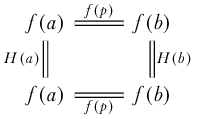
\includegraphics{./d75a6e58297fe05a808990d9551f5e2751b819cb.png}

\section{Vector fields and the Poincaré-Hopf
theorem}\label{vector-fields-and-the-poincaruxe9-hopf-theorem}
